\section*{Contexte du devoir}

\begin{figure}[h!]
    \centering
    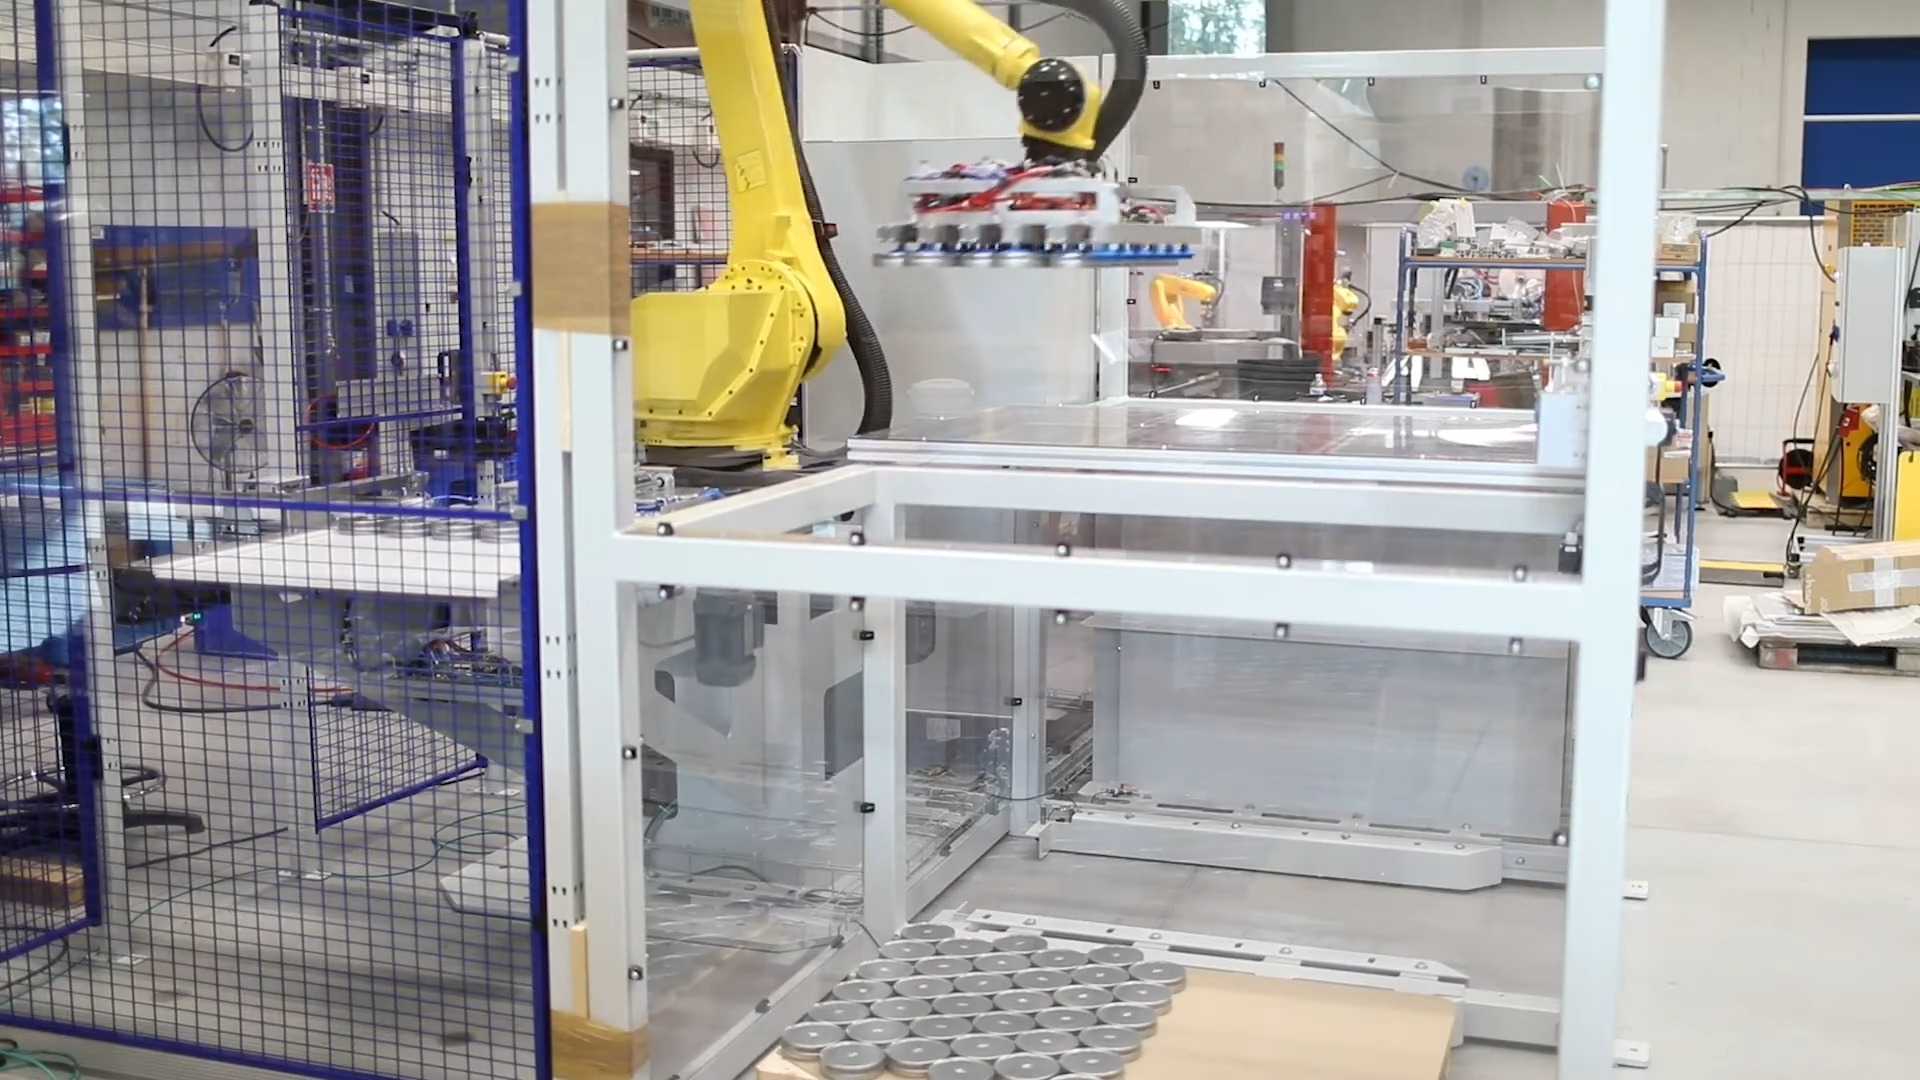
\includegraphics[width=0.7\textwidth]{figures/palletiseur}
    \caption{Cellule de palettisation automatique de boîtes}
    \label{fig:robot}
\end{figure}

\subsection*{Présentation du système}

Vous travaillez sur une cellule de \textbf{palettisation automatique de boîtes}, utilisée en fin de ligne de production pour empiler des boites de conserves conditionnés sur palette, de manière autonome.

Ler système est composé de différents sous-sytèmes : 
\begin{itemize}
    \item \textbf{Une station d'alimentation} qui achemine les boites sur une \textbf{zone tampon}.
    \item \textbf{Un robot palettiseur} qui saisit les boîtes dans la zone tampon et les dépose sur la palette selon un plan défini.
    \item \textbf{Un stock d'intercalaires}, contenant des plaques de séparation à placer entre deux couches de boîtes sur une palette.
    \item \textbf{Un changeur de palettes} qui permet de remplacer automatiquement une palette pleine.
\end{itemize}

Le système fonctionne de manière cycle selon les étapes suivantes :
\begin{enumerate}
    \item Les boîtes arrivent par lots de 6 sur un convoyeur horizontal.
    \item Chaque lot est poussé perpendiculairement vers la zone tampon, rangée après rangée.
    \item Une fois une couche complète formée, le robot palettiseur saisit les boîtes et les dépose sur la palette.
    \item Entre chaque couche, un intercalaire est placé par le robot.
    \item Une fois la palette pleine, le changeur de palettes remplace la palette pleine par une palette vide.
\end{enumerate}

Notons que le remplissage de la zone tampon se fait en parallèle des déposes des boites et des intercalaires sur la palette. Ce remplissage peut démarrer dès que le robot a soulevé les boites présentes sur la zone.  

\subsection*{Objectif du devoir}

Ce devoir surveillé porte sur la \textbf{modélisation orientée objet} et la \textbf{programmation} d'une partie de ce système. Il se concentre plus particulièrement sur :

\begin{enumerate}
    \item La conception d'une architecture objet adaptée à ce système.
    \item L'implémentation partielle de la logique du \textbf{convoyeur}.
    \item La programmation du \textbf{superviseur}, responsable de l'ordonnancement des missions.
\end{enumerate}

Vous utiliserez les conventions de nommage et les structures proposées à l'IUT. Le raisonnement objet et la capacité à structurer proprement votre code seront des éléments d'évaluation importants.